\documentclass[a4paper]{article}
\usepackage[T1]{fontenc}
\usepackage[utf8]{inputenc}
\usepackage{lmodern}
\usepackage{amsmath,amssymb}
\usepackage[top=3cm,bottom=2cm,left=2cm,right=2cm]{geometry}
\usepackage{fancyhdr}
\usepackage{esvect}
\usepackage{xcolor}
\usepackage{tikz}\usetikzlibrary{calc}

\parskip 1em\parindent 0pt

\begin{document}

\pagestyle{fancy}
\fancyhf{}
\setlength{\headheight}{15pt}
\fancyhead[L]{Optique}\fancyhead[R]{Question 12}

% Énoncé
\begin{center}
	\large{\boldmath{\textbf{Différence de marche pour un Michelson monté en lame d’air}}}
\end{center}

% Correction

\begin{center}
    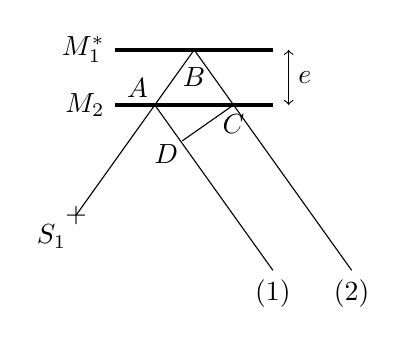
\begin{tikzpicture}[yscale=.7]
        \draw[very thick] (0,1) node[left]{$M_1^*$} -- (2,1);
        \draw[very thick] (0,0) node[left]{$M_2$} -- (2,0);
        \draw (-.5,-2) node{+} node[below left]{$S_1$} -- (1,1) node[below=3pt]{$B$} -- (1.5,0) node[below]{$C$} -- (3,-3) node[below]{(2)};
        \draw (.5,0) node[above left=-1pt]{$A$} -- (2,-3) node[below]{(1)};
        \draw (1.5,0) -- (.85,-.65) node[below left=-2pt]{$D$};
        \draw[<->] (2.2,0) -- node[right]{$e$} ++(0,1);
    \end{tikzpicture}
\end{center}
\par

Par théorème de Malus, \( \delta = AB + AC - AD \).\\
On a \( AB = BC = \dfrac{e}{\cos(i)} \) et \( AD = \sin(i) \cdot AC = 2e \cdot \sin(i)\tan(i)\).\\
\fcolorbox{red}{white}{D'où \( \delta = 2e \cdot\cos(i) \)}
\par

En présence d'une lentille mince, \(\tan(x) = \dfrac{x}{f'} \).\\
On se place proche de l'axe optique donc \( x \ll f'\).\\
\fcolorbox{red}{white}{Donc \( \delta = 2e \left(1 - \dfrac{x^2}{2f'^2}\right) \)}


\end{document}
